
% ensure we get the correct margins
% http://www.tapr.org/dcc.html#dccsubmissionguidelines
\newcommand{\CLASSINPUTtoptextmargin}{0.8in}
\newcommand{\CLASSINPUTbottomtextmargin}{1in}
\newcommand{\CLASSINPUTinnersidemargin}{0.75in}
\newcommand{\CLASSINPUToutersidemargin}{0.75in}

\documentclass[conference,letterpaper,12pt]{IEEEtran}

\usepackage{amsmath}
\usepackage{graphicx}
\usepackage[]{hyperref}
\hypersetup{
    letterpaper,
    colorlinks,
    urlcolor=blue,
    linkcolor=blue,
    citecolor=blue,
}

\usepackage[caption=false]{subfig}

\usepackage{url}
\usepackage{cite}

\bibliographystyle{IEEEtran}


% figure reference formatting
\newcommand{\figref}[1]{Fig.~\ref{#1}}

% consistent image widths
\newlength{\imgwidth}
\setlength{\imgwidth}{\columnwidth}
%\setlength{\imgwidth}{4in}


\newcommand*{\pmzeroslash}{%
    \sbox0{0}%
    \sbox2{/}%
    \sbox4{%
      \raise\dimexpr((\ht0-\dp0)-(\ht2-\dp2))/2\relax\copy2 %
    }%
    \ooalign{%
      \hfill\copy4 \hfill\cr
      \hfill0\hfill\cr
    }%
    \vphantom{0\copy4 }% correct overall height and depth of the symbol
}

%  TODO: check margins


% \IEEEauthorrefmark{1}
\author{
    \IEEEauthorblockN{Daniel J. White, Ph.D., AD\pmzeroslash CQ}
    %\IEEEauthorblockN{Daniel J. White, Ph.D., AD\O CQ}
    \IEEEauthorblockA{%
        Valparaiso University\\
        Valparaiso, Indiana\\
        \href{mailto:dan.white@valpo.edu}{dan.white@valpo.edu}}\\
    %\and
    \\
    \IEEEauthorblockN{%
        Ioannis Giannelos,
        Agisilaos Zissimatos,
        Eleytherios Kosmas,\\
        Dimitrios Papadeas,
        Pierros Papadeas,
        Matthaios Papamathaiou,\\
        Nikolaos Roussos,
        Vasileios Tsiligiannis,
        Ioannis Charitopoulos}
    \IEEEauthorblockA{%
        Libre Space Foundation\\
        Athens, Greece\\
    \href{mailto:info@satnogs.org}{info@satnogs.org}}
}

\title{SatNOGS: Satellite~Networked~Open~Ground~Station}

%TODO: add other authors



\begin{document}
\maketitle

\begin{abstract}
The SatNOGS, or Satellite Network Open Ground Stations, project promotes and supports free and open space applications.
It seeks to solve the problem of connecting many satellite users/observers to many ground station operators.
Modern open software, web, and hardware techniques are used in implementing the Network, Database, Client, and Ground Station sub-projects.
Modularity in all the systems promotes the dual-use of ground stations by not interfering with local operation while utilizing the great amount of time a civilian, non-commercial ground station would otherwise sit idle.
\end{abstract}


\begin{IEEEkeywords}
    SatNOGS, CubeSat, software-defined radio, satellite ground station, open source
\end{IEEEkeywords}

\section{Introduction}
\IEEEPARstart{T}{he} SatNOGS\cite{SatNOGS} project seeks to build a full stack of open technologies for satellite ground stations.
\IEEEPARstart{C}{ivilian} satellite launches have been in a state of change in recent years from the introduction of very small spacecraft which use standardized launch carriers such as the CubeSat and PPOD specifications \cite{WP-CubeSat}.
This has lowered the bar to satellite ownership and their availability for educational and amateur projects and citizen science.

Figure \figref{f:launches} shows that the number of CubeSat-class satellite launches has increased nearly exponentially since the first in 2000.
Previously the domain of University projects, the last 3 years have seen a huge increase in non-government or university launches.
These civilian satellites include commercial, like Planet Labs' Flock-1 satellites \cite{PlanetLabs}, non-profit, like The Planetary Society's recent LightSail \cite{PlanetarySociety}, and amateur, like AMSAT-NA's upcoming Fox-1 series \cite{AMSAT-NA}. 

\begin{figure}[htbp]
\centering
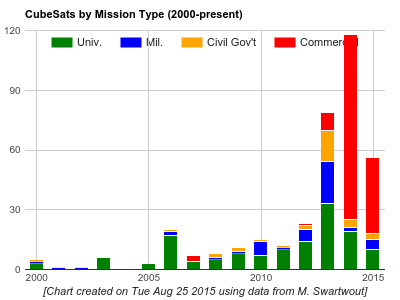
\includegraphics[width=\imgwidth]{fig/cubesat-launches}
\caption{CubeSat launches per year through 2015-07-17, from \cite{SwartwoutDatabase}.  The ``Commercial'' category includes non-profit and amateur satellites.}
\label{f:launches}
\end{figure}

Each satellite owner typically operates their own ground station for command and control.
The low-earth orbits (LEO) of these spacecraft result in short time windows when the spacecraft is above the local horizon for communication.
As a result, owners seek to enlist the help of other suitably equipped stations for collection of data.
The FUNcube project is a prime example of a well-organized effort to receive and collect data from satellite for educational outreach \cite{FUNcube}.

Recent advances in low-cost, software-defined radio (SDR) technology and 3D printing have put ground station ownership within the reach of individuals.
Largely composed of Amateur Radio operators, these people receive telemetry and data from many satellites and provide the information to the owners and the general public.

\begin{figure}[b]
\centering
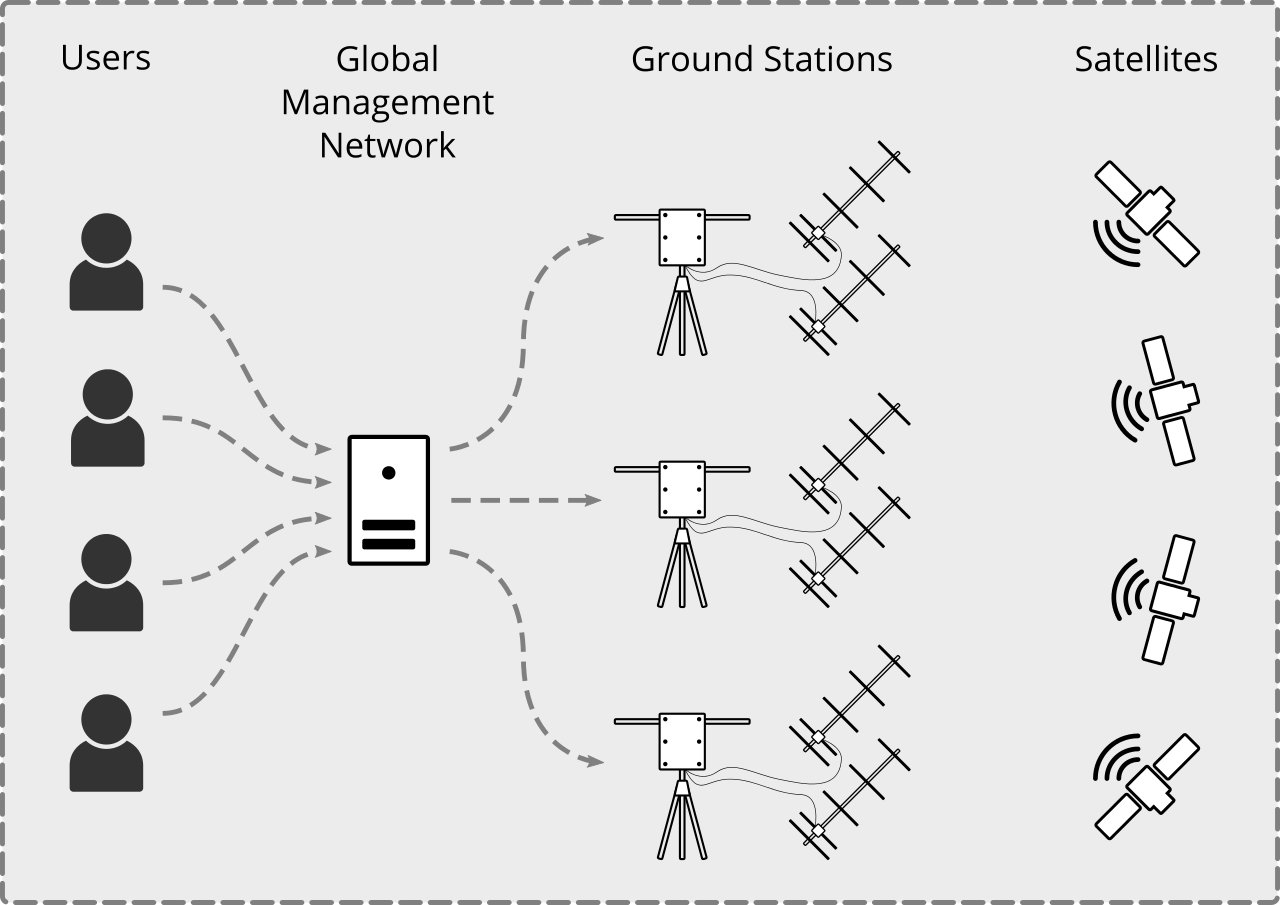
\includegraphics[width=\imgwidth]{fig/overall-system}
\caption{Overall view of the SatNOGS concept.}
\label{f:overall}
\end{figure}

Once an individual or organization builds a ground station, especially if not a commercial venture, the hardware ends up sitting idle for a great majority of the time.
This capability, when not being actively used by the local owner, could be utilized for reception of other satellites.
The SETI@Home \cite{SETI@home} project is one of the earliest and well-known projects to make use of idle resources -- computer compute cycles in that case.

What is missing is a civilian infrastructure to connect these many owners and ground station operators in a way that is flexible and open.
The ESA's Global Educational Network for Satellite Operations (GENSO) \cite{GENSO} was a notable attempt at such a network aimed at University-class projects and stations.
The fact that the \verb|genso.org| domain name does not resolve to a live server is practical indication of the current state of the project.

Members of \emph{Hackerspace.gr} \cite{Hackerspacegr} in Athens Greece first proposed SatNOGS as a part of the 2014 International Space Apps Challenge's ``Virtual Ground Station App -- Global Crowdsourcing of CubeSats'' Challenge \cite{SpaceAppsChallenge2014-SatNOGS}.
It was later submitted as an entry to the 2014 Hackaday Prize \cite{HackadayPrize2014}, ultimately winning the grand prize of $\$196,418$.
The funds provided seed money to start the Libre Space Foundation \cite{LibreSpaceFoundation}, a new non-profit dedicated to supporting free and open source space and related projects.

A timely and unique aspect of the project is its bridging of the Maker / Hacker and the Amateur Radio communities.
The 2015 TAPR/AMSAT Banquet's speaker, Michael Ossmann AD\pmzeroslash NR pointed out the many characteristics valued and shared by these two communities \cite{HamRadioNow211}.
Ward Silver's article for Makezine also does a good job of drawing these connections \cite{Silver2015}.

% TODO: \cite{SatNOGS-Hamvention2015}

This paper seeks to give an overview of the SatNOGS project's major components.
Figure \figref{f:overall} gives a high-level overview of the relationship between users and ground stations.
Figure \figref{f:modular} and the following sections describe the four major sub-projects: Network, DB, Client, and Ground Station.
The modular approach maximizes use of already available components at a ground station.

\begin{figure}[b]
\centering
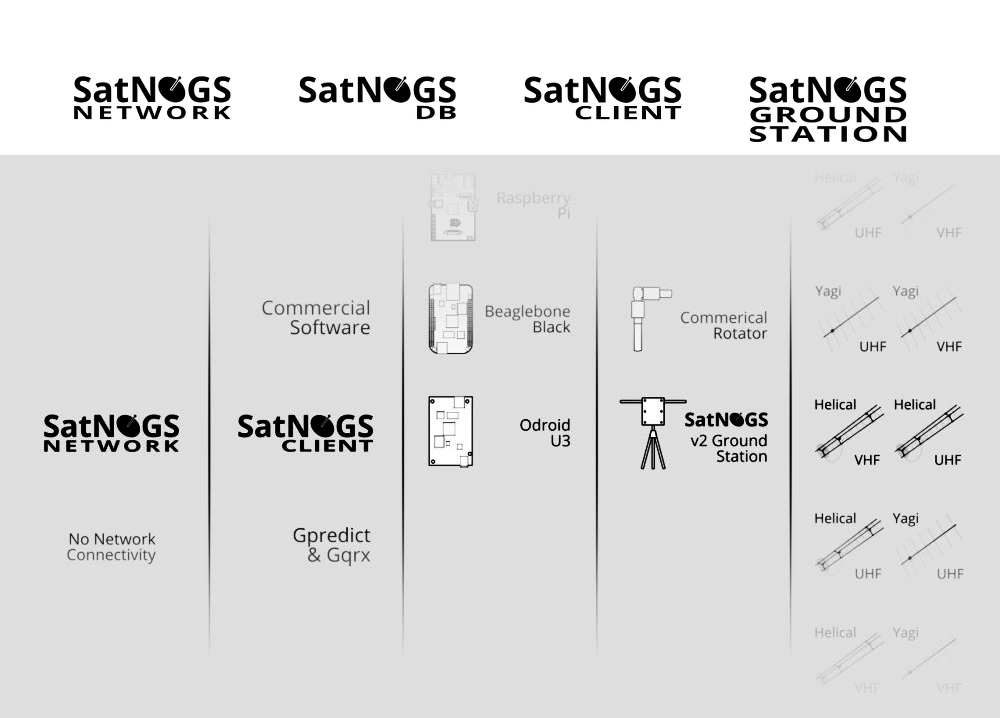
\includegraphics[width=\imgwidth]{fig/components-modular}%
\caption{The four sub-projects are designed with a modular approach with well-defined interfaces, allowing the ability to relatively easily interface with existing ground stations.}
\label{f:modular}
\end{figure}

All code and hardware designs for the project are publicly available \cite{SatNOGS-github} under Open Software (AGPLv3 and GPLv3) and Open Hardware (CERN OHLv1.2) licenses.
Software documentation may be found at \cite{SatNOGS-docs}.
Note, screen captures of the various software components, hardware pictures, and demonstrations are included in the more appropriate format of the presentation instead of in the paper.


\section{Network}
The SatNOGS Network is accessed by users via a web interface.
The user provides details about observation that they would like to schedule (which satellite, which band, time-frame, signal encoding, etc.).
From this information, the system calculates the possible observation windows from the currently available Ground Stations (GS) connected to the Network with the necessary capabilities.
Once the observer confirms the proposed ``observation job'' then it is sent as a job to each Ground Stations' job queue to be executed.
Figure \figref{f:network} shows this process as a diagram.

\begin{figure}[htbp]
\centering
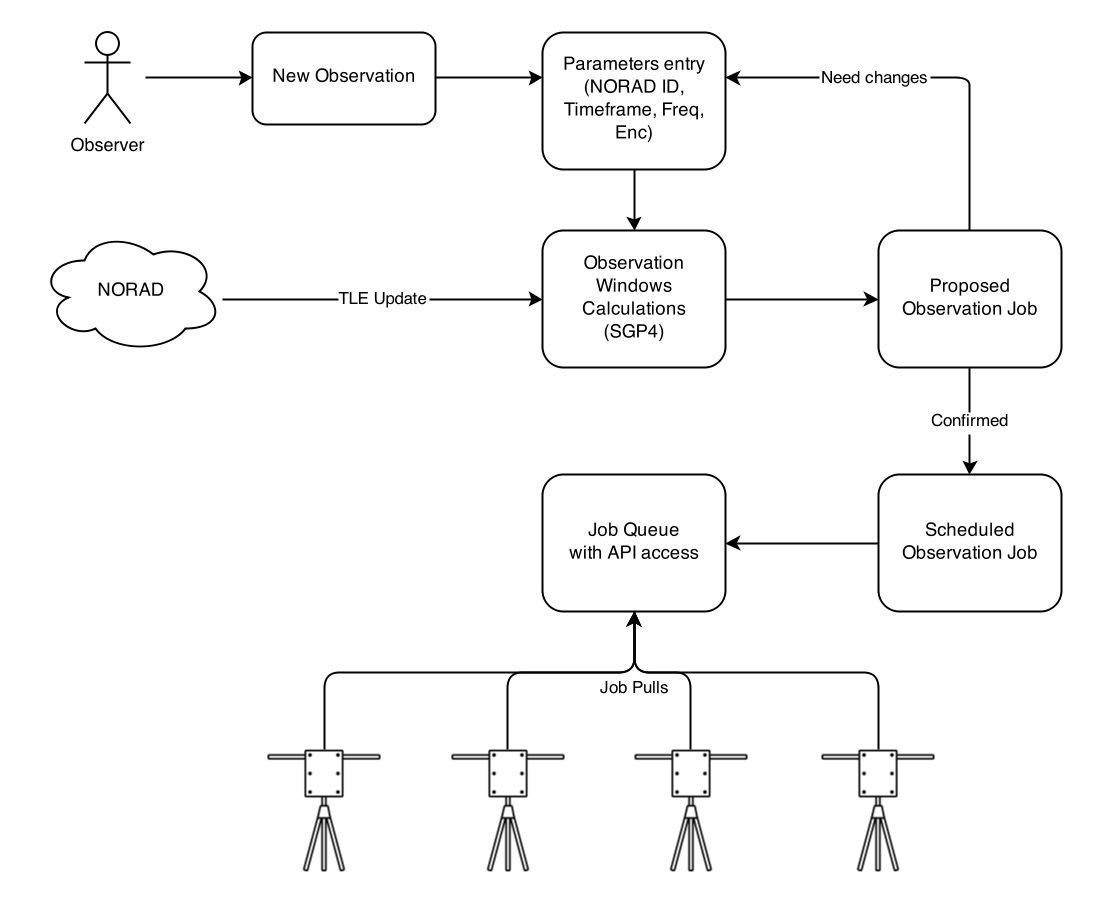
\includegraphics[width=\imgwidth]{fig/network-flow}
\caption{Diagram of a user scheduling an observation on the network.}
\label{f:network}
\end{figure}

Ground Stations then collect and send observation data back to the Network.
Uploaded data is then made available to the initiating user and any other third party via the observation's ID.
Modern web technologies are used on the Network website to provide timeline and recording visualization and playback directly in the browser.
Download links are also provided for further offline analysis.
No special software or installation is necessary for users to interact with the Network.
SatNOGS Network provides an API to allow other applications and services to query information and, in the future, automatically schedule observations.

Calculation of candidate times when the target satellite is visible from an active ground station is performed with the assistance of the PyEphem library \cite{PyEphem}.
The library accepts orbital elements for the satellite, Ground Station locations, and the desired time frame.
With higher densities of Ground Stations which can see multiple satellites, this scheduling can be optimized for many factors.

Because all code and documentation of all parts of the project are free and publicly available, anyone is able to contribute to these improvements.
Indeed, this open collaboration is one of the SatNOGS project's founding principles.


\section{Database}
The centralization provided by the Network component requires a centralized source of satellite information such as frequencies and transmission modes.
SatNOGS DB was created to address the fact that there was no known public source for this information.
In the same spirit of the rest of the project, the database is open access and not specific only to the SatNOGS project.

Specifically, DB is a crowd-sourced suggestions app for transponder data.
Satellites are identified by their NORAD (now USSPACECOM) space object catalog number and their common name.
Each object has an associated set of transponder records which indicate frequencies and modulation formats.
SatNOGS Network pulls this information when calculating possible observations.

Updates are accepted from the public and from other sources of satellite information with open APIs.
As with the Network, user interaction is purely web-based and requires no additional software beyond a capable browser.


\section{Client}
SatNOGS Client consists of software running a computer which controls the ground station hardware.
Figure \figref{f:client-flow} diagrams the internal (modular!) components of the client's interaction with the Network.

\begin{figure}[htbp]
\centering
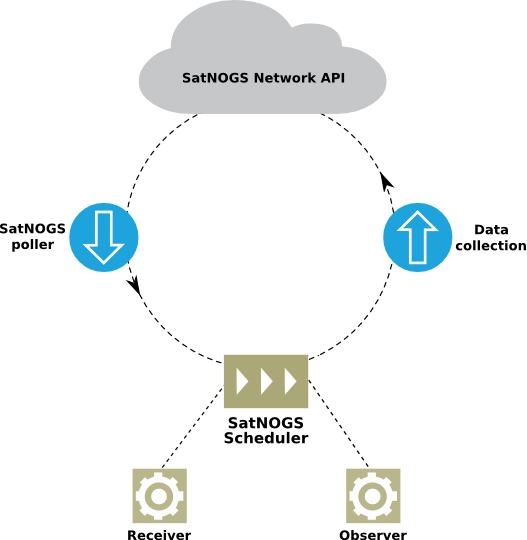
\includegraphics[width=\imgwidth]{fig/client-flow}
\caption{Client software components and interactions.}
\label{f:client-flow}
\end{figure}

The poller regularly checks the Network API for observation jobs scheduled for the local Ground Station.
Information contained in each job includes satellite orbital elements, receiver tuning and demodulation parameters, and timing.
The PyEphem \cite{PyEphem} library is used to calculate the necessary antenna pointing and relative velocity for doppler shift calculation during the pass.

Where possible, existing standard interfaces are used within the Client.
These include using the daemons \verb|rotctl| for rotator control and \verb|rigctl| for frequency control from HamLib \cite{Hamlib}.
Any rotator controller which works with \verb|rotctl| automatically works with the SatNOGS Client by providing the appropriate IP address and port number the rotator is listening on.

External programs for starting the receiver driver are spawned before a scheduled observation and setup to listen for \verb|rotctl| commands for doppler frequency corrections throughout a pass.
For use with the popular Realtek RTL2832U DVB-T dongles, the SatNOGS group maintains a version of \verb|rtl-sdr| \cite{rtl-sdr} software's \verb|rtl_fm| utility which accepts frequency control via \verb|rigctl| commands over a network port \cite{SatNOGS-rtlsdr}.
Code for interfacing the Client with other SDR software is in progress, including receivers using GNU Radio \cite{GNURadio}.
Radios whose baseband signals enter the computer via soundcard are also planned.

At the end of a pass, demodulated signal data is placed in a queue for later upload to the Network.
Logs and other reports are also sent back to the Network by other API actions.


\section{Ground Station}
The SatNOGS Ground Station sub-project encompasses the antennas, rotator, and RF path.
Ground station owners execute the Client software and build or configure the hardware.
Plans and instructions are available for the v2 ground station and are being finalized for the updated v3 version.
Gears and other parts are 3D printed and the rest of the hardware for the ground station is easily available.
Besides access to a 3D printer, only hand tools are required for building either version.

Because the Ground Station rotator's controller implements the common EasyComm 2 protocol, it acts like any other homebrew or commercial rotator controller using the same format.
The Client software therefore works exactly the same with the SatNOGS rotator design or with an existing station's rotator.

There are designs for every component necessary for a SatNOGS-compatible ground station as part of the project.
Antennas and RF path hardware may be use SatNOGS, homebrew, or commercial as the station owner deems appropriate.
To help the goal of easily constructed ground stations, the project's designs focus on common hardware, 3D-printed parts, and tools available in most experimenters' shops of local ``maker spaces.''


\section{Conclusion}
The SatNOGS project aims to provide and promote free and open source satellite ground stations.
Modern open software and web technologies are used to coordinate these stations to more fully utilize the reception capabilities for low earth orbiting satellites.
By using a modular approach to the ground station segment, the existing stations of radio amateurs and others may be used with the network.
Avoiding custom, network-specific software and hardware and ensuring all design information, code, and received data is and remains freely available is a core tenet of the project.
Individuals and organizations are encouraged to partner with the project to help realize these goals.

\bibliography{references}

\end{document}
% vim: spell wrap linebreak textwidth=0
